\section{Calorimeter}

The calorimeter system fulfils several primary roles in the LHCb detector. It provides very fast measurements which are used by the trigger to make quick judgements on an event (a decision is made 4 microseconds after the interaction); examples of such measurements are,

\begin{itemize}
	\item $E_T$ of electrons, photons and neutral pions 
	\item $E_T$ and $\Sigma(E_T)$ of Hadrons
\end{itemize}

As well as providing fast information it also provides information on the particle type, discriminating between electrons, photons and hadrons. It is especially useful at identifying neutral particles such as photons and neutral mesons, e.g. pions. This enables the LHCb detector to make  physics measurements for many decays, see table \ref{table: calorimeter processes},
\\
\begin{table}[h]
	\begin{center}
		\begin{tabular}{ |l|l| }
		%	\hline
		%	\multicolumn{2}{ |c| }{Calorimeter Particle Identification} \\
			\hline
			Particle Type & Example Process \\ \hline
			Electron & $B \rightarrow K* e^+ e^-$ \\ \hline
			\multirow{2}{*}{Photons} & $B_d \rightarrow K* \gamma$ \\
				 & $B_s \rightarrow \phi \gamma$ \\ \hline
			\multirow{2}{*}{Neutral Mesons} & $B_d \rightarrow \pi^+\pi^-\pi^0$ \\
				 &  $B_d \rightarrow J/\psi \eta$ \\ \hline
		\end{tabular}
		\caption{Calorimeter particle identification}
		\label{table: calorimeter processes}
	\end{center}
\end{table}

The calorimeter system is positioned approximately thirteen metres downstream of the nominal interaction point with a solid angle coverage of 300 mrad in x and 250 mrad in y \cite{Amato:494264}. It extends for 2.7 metres (See figure \ref{fig: lhcb_schematic}) and is composed of several sub-components. In order of distance from the nominal interaction point these are the Scintillating Pad Detector (SPD), a 2.5 radiation length ($2.5\,X_0 = 12$~mm) lead wall, the Pre Shower (PS), an electromagnetic calorimeter (ECAL) with dimensions of 4 m x 3.5 m and a hadronic calorimeter (HCAL). Each component is designed to maximise the signal of certain particle types and minimise the signal for others. The nominal signal deposition regions for various particle types are shown in figure \ref{fig:animals}

\begin{figure}[h]
        \centering
        \begin{subfigure}[b]{0.5\textwidth}
                \centering
                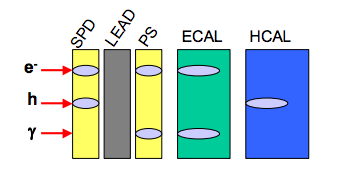
\includegraphics[width=\textwidth]{./Chapters/detector/calorimeter/deposition_region.png}
                \label{fig: calo_nominal_detection_regions1}
                \caption{}
        \end{subfigure}
        \begin{subfigure}[b]{0.4\textwidth}
                \centering
                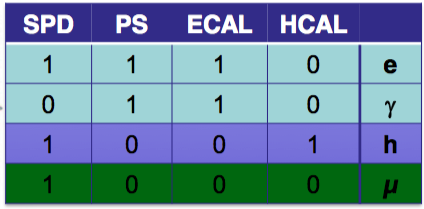
\includegraphics[width=\textwidth]{./Chapters/detector/calorimeter/deposition_region_table.png}
                \label{fig: calo_nominal_detection_regions2}
                \caption{}
        \end{subfigure}
        \caption{(A): Nominal regions of energy deposition in the LHCb calorimeter system for various particle types (B): Nominal particle signal detection in the LHCb calorimeter system for various particle types}
        \label{fig:animals}
\end{figure}

\begin{figure}[h]
	\centering
	\begin{subfigure}[b]{0.45\textwidth}
		\centering
		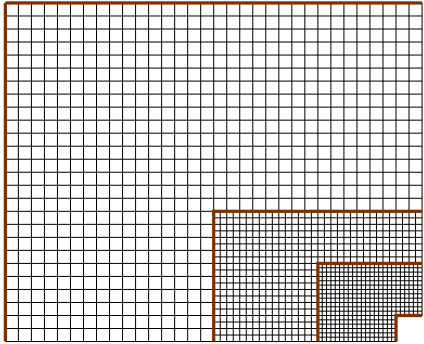
\includegraphics[width=\textwidth]{./Chapters/detector/calorimeter/ecal_graularity.png}
		\caption{ECAL}	
		\label{fig: ECAL granularity}
	\end{subfigure}
	\begin{subfigure}[b]{0.45\textwidth}
		\centering
		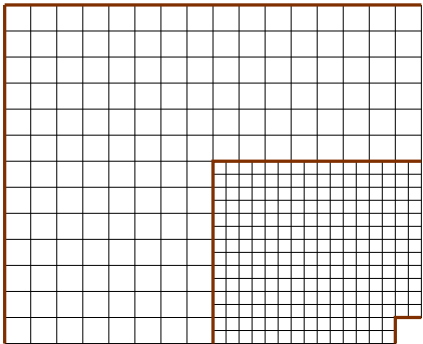
\includegraphics[width=\textwidth]{./Chapters/detector/calorimeter/hcal_granularity.png}
		\caption{HCAL}	
		\label{fig: HCAL granularity}
	\end{subfigure}
	\caption{Schematic of the cell granularity of the LHCb calorimeters for one of its quadrants. See tables \ref{table: Calorimeter details} and \ref{table: Calorimeter details2} for further details.}
\end{figure}

\begin{table}[htdp]
	\caption{Cell granularity structure of the SPD/PS and ECAL components of the LHCb calorimeter system}
	\begin{center}
		\begin{tabular}{|c|c|c|c|}
			\hline
			& Inner region & Middle region & Outer region \\
			\hline
			Cell size (mm) & 40.4 & 60.6 & 121.2 \\
			\hline
			Number of channels & 1472 & 1792 & 2688 \\
			\hline
		\end{tabular}
	\end{center}
	\label{table: Calorimeter details}
\end{table}%

\begin{table}[htdp]
	\caption{Cell granularity structure of the HCAL component of the LHCb calorimeter system}
	\begin{center}
		\begin{tabular}{|c|c|c|}
			\hline
			& Inner region & Outer region \\
			\hline
			Cell size (mm) & 131.3 & 262.6 \\
			\hline
			Number of channels & 860 & 680 \\
			\hline
		\end{tabular}
	\end{center}
	\label{table: Calorimeter details2}
\end{table}%


The SPD and PS are made from scintillator pads and contain a groove which holds a helicoidal optical fibre that collects scintillating light. The ECAL is a Shashlik electromagnetic calorimeter, it is made of interleaved tiles of 2mm think lead absorbers and 4mm thick scintillator material orientated to face the direction of the beam pipe; there are 66 of these interleaved pairs of lead and scintillator tiles giving a longitudinal size of 25 radiation lengths ($X_0$). The HCAL is made of interleaved plates of Scandium and Iron and is orientated in the horizontal plane. It has a longitudinal size of 5.6 hadron interaction lengths ($\lambda_I$) and is made up of 26 layers of Scandium and Iron plate pairs.

From beam tests \cite{1742-6596-293-1-012052} the ECAL has been shown to have an energy resolution of,
\begin{equation*}
	\frac{\sigma_E}{{E}} = \frac{(8-10)\%}{\sqrt{E}} \oplus 0.9\%
\end{equation*}

and the HCAL has been shown to have a resolution of 
\begin{equation*}
	\frac{\sigma_E}{E} = \frac{69\pm5\%}{\sqrt{E}} \oplus 9\pm2\%
\end{equation*}

%Figure \ref{fig: reconstruction using calorimeter} shows examples of particle reconstruction using information from the calorimeter system.
Figure \ref{fig: reconstruction using calorimeter} shows the invariant masses of particles reconstructed using hits in the calorimeter system.

\begin{figure}
	\centering
	\begin{subfigure}[b]{0.42\textwidth}
		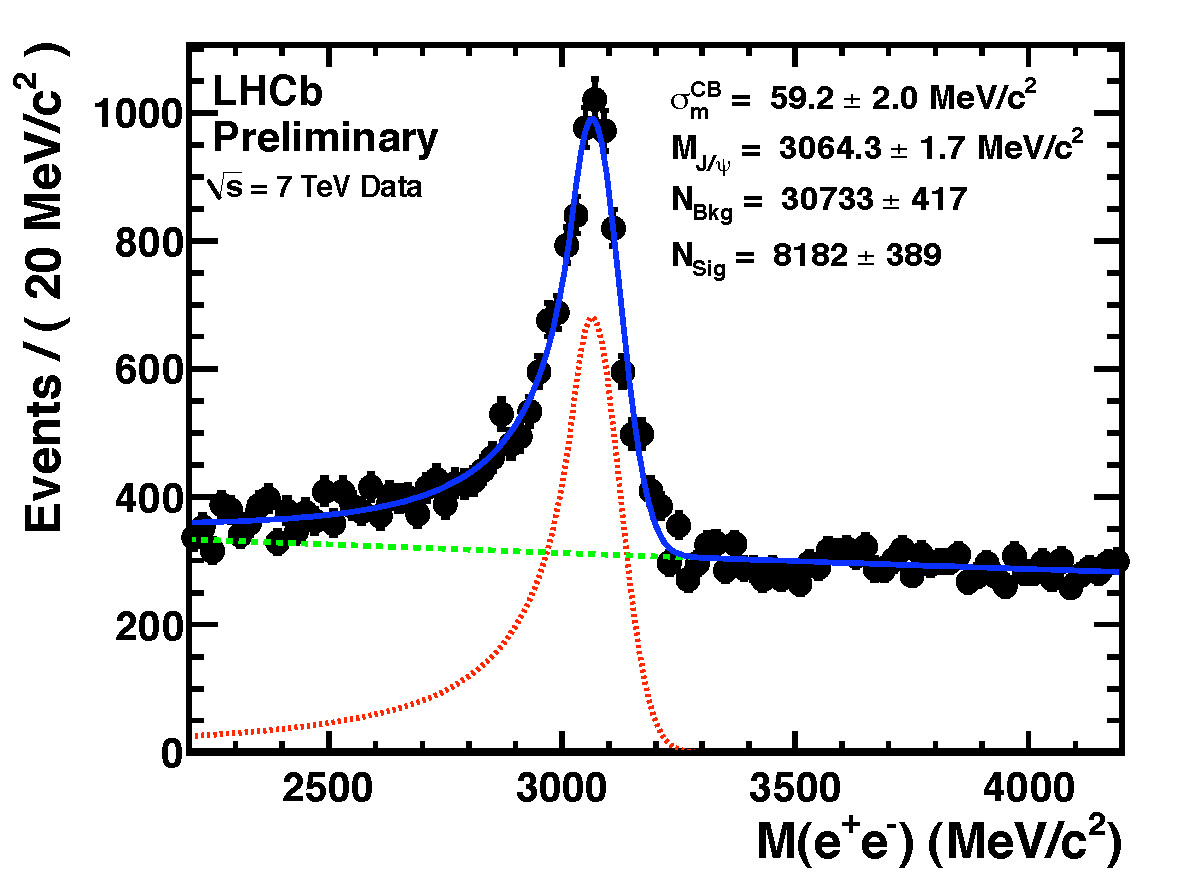
\includegraphics[width=\textwidth]{./Chapters/detector/calorimeter/jpsi_to_ee.pdf}
		\caption{}
	\end{subfigure}
	\begin{subfigure}[b]{0.46\textwidth}
		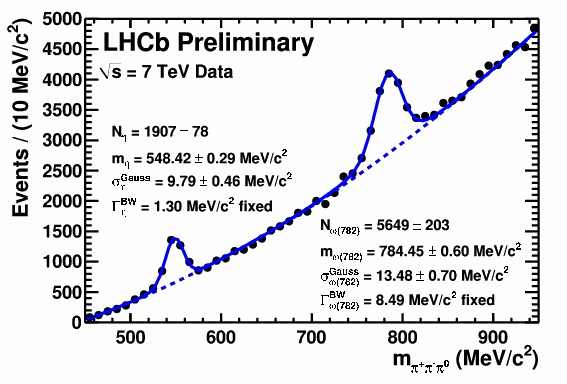
\includegraphics[width=\textwidth]{./Chapters/detector/calorimeter/eta_omega_pipipi_reconstruction.jpg}
		\caption{}
	\end{subfigure}
	\caption{Reconstruction of (A) $J/\psi \rightarrow e^+e^-$} and (B) $\eta/\omega \rightarrow \pi^+\pi^-\pi^0$ using information from the calorimeter system.
	\label{fig: reconstruction using calorimeter}
\end{figure}
